\documentclass[12pt]{beamer}
\usetheme{LMT}
\usepackage[utf8]{inputenc}
\usepackage{amsmath}
\usepackage[makeroom]{cancel}
\usepackage{xcolor}
\usepackage[absolute,overlay]{textpos} %[showboxes,absolute,overlay]{textpos}
\usepackage[nomessages]{fp} % Calcul simple avec  \FPeval{
\usepackage{tikz}


\setbeamertemplate{footline}[frame number]{}

\makeatletter
\newcommand*{\overlaynumber}{\number\beamer@slideinframe}
\makeatother

\newcommand\Ccancel[2][black]{\renewcommand\CancelColor{\color{#1}}\bcancel{#2}}

\newcommand\encircleR[1]{%
  \tikz[baseline=(X.base)] 
    \node (X) [draw, shape=circle, inner sep=0,minimum size=1cm, color=red, line width=1.5] {\strut #1};}
    
\newcommand\encircleG[1]{%
  \tikz[baseline=(X.base)] 
    \node (X) [draw, shape=circle, inner sep=0,minimum size=1cm, color=green, line width=1.5] {\strut #1};}
    
\newcommand\encircleB[1]{%
  \tikz[baseline=(X.base)] 
    \node (X) [draw, shape=circle, inner sep=0,minimum size=1cm, color=blue, line width=1.5] {\strut #1};}
    
\newcommand\encircleK[1]{%
  \tikz[baseline=(X.base)] 
    \node (X) [draw, shape=circle, inner sep=0,minimum size=1cm, color=black, line width=1.5] {\strut #1};}

\newcommand\encircledR[1]{%
  \tikz[baseline=(X.base)] 
    \node (X) [draw, shape=circle, inner sep=0,minimum size=1cm, color=red, dashed, line width=1.5] {\strut #1};}
    
\newcommand\encircledG[1]{%
  \tikz[baseline=(X.base)] 
    \node (X) [draw, shape=circle, inner sep=0,minimum size=1cm, color=green, dashed, line width=1.5] {\strut #1};}
    
\newcommand\encircledB[1]{%
  \tikz[baseline=(X.base)] 
    \node (X) [draw, shape=circle, inner sep=0,minimum size=1cm, color=blue, dashed, line width=1.5] {\strut #1};}
    
\newcommand\encircledK[1]{%
  \tikz[baseline=(X.base)] 
    \node (X) [draw, shape=circle, inner sep=0,minimum size=1cm, color=black, dashed, line width=1.5] {\strut #1};}
    

\pdfinfo
{
  /Title       (Presentation Reunion)
  /Author      (Pierre NARGIL)
}

\newcommand\FontReduce{\fontsize{8}{10}\selectfont}
\newcommand\FontReduceT{\fontsize{9}{11}\selectfont}


\title{Avancement du travail}
\subtitle{Présentation hebdomadaire}
\author{Pierre Nargil}

\graphicspath{{figures/}}
% ---------------------------------------------------------------------
\begin{document}


\frame{\titlepage}

\frame{\tableofcontents}


\section{Rappels de la dernière réunion}

	\begin{frame}
	
		\frametitle{Rappels de la dernière réunion}
		%\framesubtitle{Un sous titre}
		
		\begin{itemize}
%			\item Les questions abordées :
%			\begin{itemize}
%				\only<1>{\FontReduce}
%				\item Expliquer la différence sur le cas analytique
%						\\ 	\only<2>{\textcolor{blue}{Évolution du programme de François depuis la présentation.}}
%				\item \textcolor<-1>{red}{Pour réutiliser les modes trouvés par SVD, comment trouver les fonctions en temps associées ?}
%						\\ 	\only<3>{\textcolor{blue}{...}}
%				\item \textcolor<-1>{red}{Le 1er mode de la 1ère itération est-il  la répose statique dde l'effort moyen ?}
%			\end{itemize}
			
				\item Les objectifs de travail à court terme :
				\begin{itemize}
					\FontReduce
					%\item \textcolor<-1>{red}{Differente fréquences F(t) (comparer aux f propre de la poutre) $\Rightarrow$ quand ça diverge
					%		(Somme de sinus à la place de SinusVerse ?)}
					\only<1,2>{\item $[M]$ et $[K]$ diagonale dans la base POD ?} 
					\only<2>{\\
						$
						Mr = 10^{-4} *
						\begin{bmatrix}
						   24.1738 &  -0.2296 &   0.0071  &  0.2178  \\
						   -0.2296  & 24.1091 &   0.0058  &  0.2493 \\
						    0.0071  &  0.0058 &  24.3384 &  -0.0158 \\
						    0.2178  &  0.2493 &  -0.0158 &  24.1268 \\
						\end{bmatrix}
						$
						\\
						$ 
						Kr = 10^5 *
						\begin{bmatrix}
						    7   &  6  &   0 &   -5 \\
						     6  &  68 &   38 &  -15 \\
						     0  &  38 &  602  & 134 \\
						    -5  & -15 &  134 &  209
						\end{bmatrix}
						$
						\\
						Non, mais je tente tout de même d'utiliser les coefficients diagonaux dans les slides suivantes.
						}
					\only<1,3,4,5,6>{\item Évaluer dans le problème en temps évaluer les termes "m" et "k" }
						\only<3,4,5,6> {
						$
						\sqrt{Kr(i,i)/Mr(i,i)} = 10^5 *
						$
						\\
						$ \!\!\!\!\!\!\!\!\!\!\!\!\!\!\!\!\!\!\!\!\!\!\!\!\!\!\!\!\!\!
						\begin{Bmatrix}
						0.1708,~  0.5297,~  1.5721,~  0.9307,~  1.6381,~  1.2988,~  2.6629,~  3.0521,~  3.3865,~  3.7222 
						\end{Bmatrix} \!\!\!\!\!\!\!\!\!\!\!\!\!\!\!\!\!\!\!\!\!\!\!\!\!\!\!\!\!\!
						$
						}
						\only<3>{
						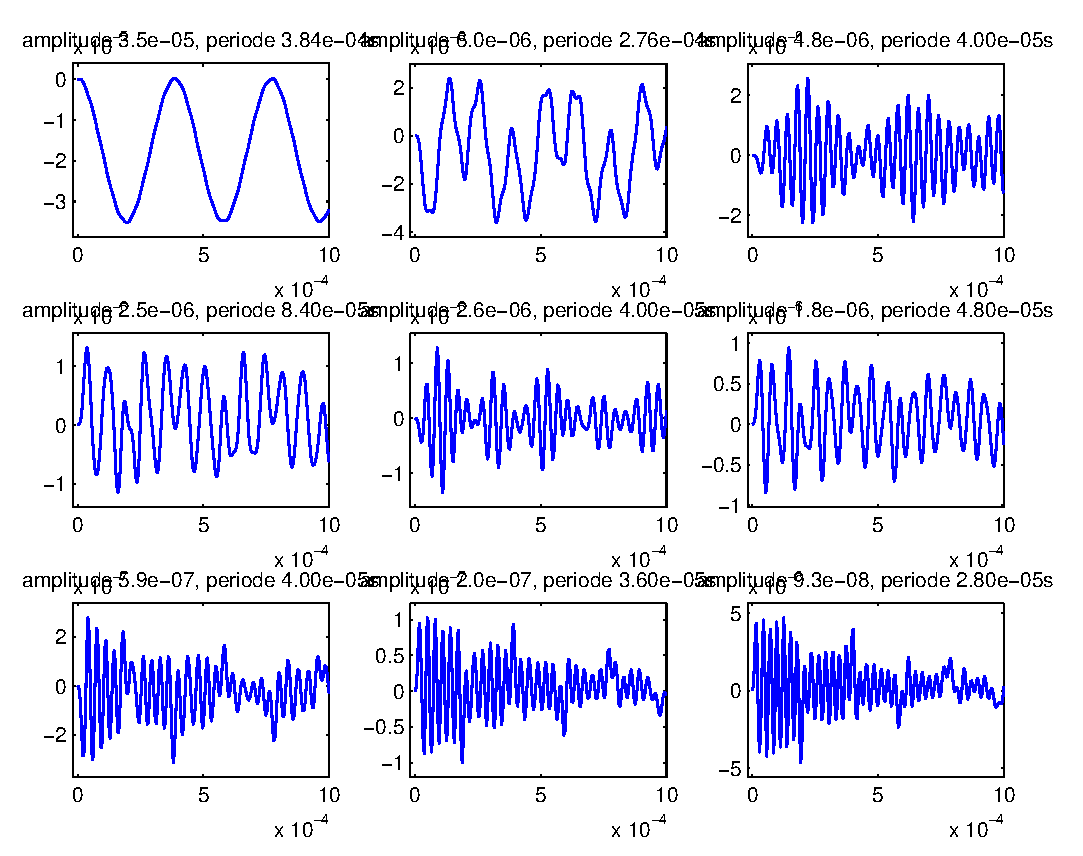
\includegraphics[width=0.8\linewidth ,keepaspectratio]{matPODModesTemps-diverg.eps}
						\\
						On observe une certaine corrélation entre l'évolution du "$\omega_0$"
						et l'évolution des fréquences des modes en temps de la POD.
						}
						\only<4>{
						\begin{figure}
							\hspace{-2cm}
							\begin{minipage}{0.25\linewidth}
								\textcolor{red}{Résultats POD}
								\\
								\textcolor{blue}{$\frac{\sqrt{K/M}}{2*\pi}$ POD }
							\end{minipage}
							\begin{minipage}{0.3\linewidth}
								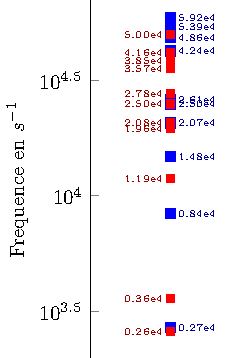
\includegraphics[height=6cm ,keepaspectratio]{Tikz/Frise3/Freq.pdf} 
							\end{minipage}
						\end{figure}
						\begin{textblock}{6}[0,0](2,12)
							Ici on peut visualiser un peu mieux et comparer $\omega_0$ 
							et les fréquences des premiers modes.
						\end{textblock}
						}
						\only<5>{
						\begin{figure}
							\hspace{-2cm}
							\begin{minipage}{0.25\linewidth}
								\textcolor{red}{Résultats POD}
								\\
								\textcolor{blue}{$\frac{\sqrt{K/M}}{2*\pi}$ POD }
							\end{minipage}
							\begin{minipage}{0.3\linewidth}
								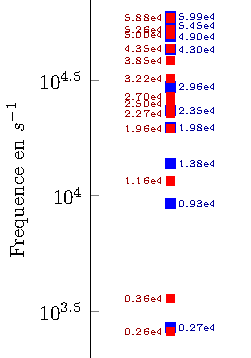
\includegraphics[height=6cm ,keepaspectratio]{Tikz/Frise4/Freq.pdf} 
							\end{minipage}
						\end{figure}
						\begin{textblock}{6}[0,0](2,12)
							Même chose avec une discrétisation temporelle plus fine
						\end{textblock}
						}
						\only<6>{
						\\
						$ \!\!\!\!\!\!\!\!\!\!\!\!\!\!\!\!\!\!\!\!\!\!\!\!\!\!\!\!\!\!
						\begin{Bmatrix}
						1.6537,~   0.1728,~  1.6678,~   1.7965,~   1.5097,~   1.5219,~   1.5919,~   1.5591,~   1.5615,~   1.6244
						\end{Bmatrix} \!\!\!\!\!\!\!\!\!\!\!\!\!\!\!\!\!\!\!\!\!\!\!\!\!\!\!\!\!\!
						$
						%\end{itemize} 
						\\
						}
						\only<6>{
						\begin{figure}
						\hspace{-2cm}
							\begin{minipage}{0.25\linewidth}
								\textcolor{red}{$\sqrt{K/M}$ PGD}
								\\
								\textcolor{blue}{$\sqrt{K/M}$ POD}
							\end{minipage}
							\begin{minipage}{0.3\linewidth}
								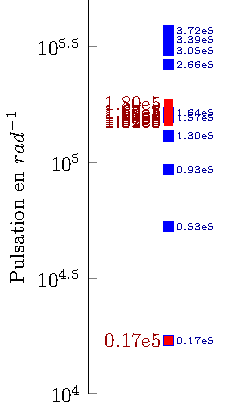
\includegraphics[height=6cm ,keepaspectratio]{Tikz/Frise2/Freq.pdf} 
							\end{minipage}
						\end{figure}
						\begin{textblock}{6}[0,0](2,6)
							On compare avec le $\omega_0$ obtenu grâce aux "m" et "k" du problème en temps PGD, 
							sur un exemple où la PGD diverge, puisque dans la discussion avec François Vendredi dernier,
							on cherchait à imputer la responsabilité de la divergence à des mauvais couples "m" et "k"
						\end{textblock}
						\begin{textblock}{6}[0,0](2,11.5)
							Ce que l'on peut remarquer c'est que, pour le mode le plus pertinent trouvé par la PGD (trouvé en $2^e$),
							le point fixe converge vers un $\omega_0$ correspondant à celui évalué pour le premier mode POD.
							Tous les autres points fixes vont vers une valeur d'$\omega$ similaire.
						\end{textblock}
						}
					\only<1,7>{\item Faire une frise des freq propre et freq d'excitation}
						\only<7>{\\
						\begin{figure}
						\hspace{-2cm}
							\begin{minipage}{0.2\linewidth}
								\textcolor{red}{Chargement}
								\\
								\textcolor{blue}{F propres}
							\end{minipage}
							\begin{minipage}{0.5\linewidth}
								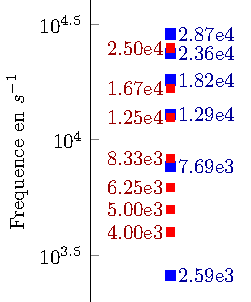
\includegraphics[height=6cm ,keepaspectratio]{Tikz/Frise/Freq.pdf} 
							\end{minipage}
						\end{figure}
						\begin{textblock}{5}[0,0](1.5,5)
							Je m'étais un peu emmêlé les pinceaux la dernière fois, en image c'est plus clair. 
							Le chargement avec les trois fréquences les plus basses on a une sollicitation "gentille".
						\end{textblock}
						}
					\only<1,8>{\item Tester convergence de la PGD vers la solution direct avec dt petit}
						\only<8>{
							\begin{itemize}
								\item Utilisation du cluster
							\end{itemize}
							}
					\only<1>{\item \textcolor<-1>{red}{Trouver le C critique du probleme poutre (liaison avec la longueur des éléments ?)}}
					\only<1>{\item \textcolor<-1>{red}{Rôle du $dt$ different entre PGD et Methode directe}}
					\only<1>{\item \textcolor<-1>{red}{Est-il possible de raffiner en temps après n modes}}
					\only<1>{\item \textcolor<-1>{red}{comparer freq des modes POD/PGD}}
					\only<1>{\item \textcolor<-1>{red}{Comparer avec la solution exacte}}
					\only<1>{\item \textcolor<-1>{red}{littérature SVD(PGD) }}
					%\only<1,2,3,5,6> {
				\end{itemize}  % }
		\end{itemize}

	\end{frame}
	
	\begin{frame}
	
		\frametitle{Rappels de la dernière réunion}
		%\framesubtitle{Un sous titre}
		
		\begin{itemize}
%			\item Les questions abordées :
%			\begin{itemize}
%				\only<1>{\FontReduce}
%				\item Expliquer la différence sur le cas analytique
%						\\ 	\only<2>{\textcolor{blue}{Évolution du programme de François depuis la présentation.}}
%				\item \textcolor<-1>{red}{Pour réutiliser les modes trouvés par SVD, comment trouver les fonctions en temps associées ?}
%						\\ 	\only<3>{\textcolor{blue}{...}}
%				\item \textcolor<-1>{red}{Le 1er mode de la 1ère itération est-il  la répose statique dde l'effort moyen ?}
%			\end{itemize}
			
				\item Les objectifs de travail à court terme :
				\begin{itemize}
					\FontReduce
					\only<1,2>{\item
						$
						Mr = 10^{-4} *
						\begin{bmatrix}
						   24.2 &  0.28 &   0.31  &  -0.30  \\
						   .  & 23.9 &   -0.52  &  0.51 \\
						    .  &  . &  23.8 &  -0.0158 \\
						    .  &  . & . &  23.8 \\
						\end{bmatrix}
						$
						\item 
						$ 
						Kr = 10^5 *
						\begin{bmatrix}
						    6.51   &  -2.48  &   -3.27 &   3.19 \\
						     .  &  89.4 &   86.3 &  -85 \\
						     .  &  . &  294  & -236 \\
						    .  & . &  . &  543
						\end{bmatrix}
						$
						\\
						Encore mois qu'avant.
						}
						
					\only<1,3,4,5,6>{\item Évaluer dans le problème en temps évaluer les termes "m" et "k" }
						\only<3,4,5,6> {
						$
						\sqrt{Kr(i,i)/Mr(i,i)} / 2.pi = 10^5 *
						$
						\\
						$ \!\!\!\!\!\!\!\!\!\!\!\!\!\!\!\!\!\!\!\!\!\!\!\!\!\!\!\!\!\!
						\begin{Bmatrix}
						0.261,~  0.973,~  1.77,~  2.40,~  3.02,~  3.64,~  4.26,~  4.85,~  5.43,~  5.99 
						\end{Bmatrix} \!\!\!\!\!\!\!\!\!\!\!\!\!\!\!\!\!\!\!\!\!\!\!\!\!\!\!\!\!\!
						$
						}
						\only<3>{
						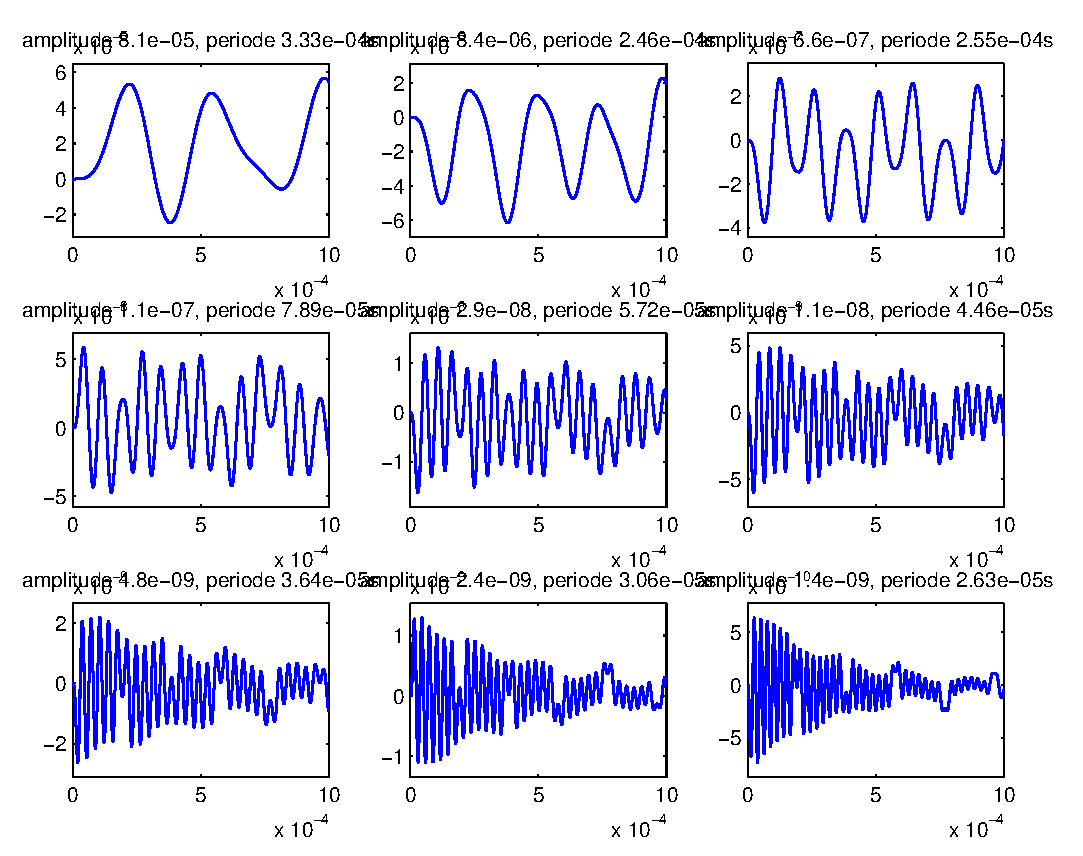
\includegraphics[width=0.8\linewidth ,keepaspectratio]{matPODModesTemps-diverg-dt5.eps}
						\\
						On observe une certaine corrélation entre l'évolution du "$\omega_0$"
						et l'évolution des fréquences des modes en temps de la POD.
						}
						\only<4>{
						\begin{figure}
							\hspace{-2cm}
							\begin{minipage}{0.25\linewidth}
								\textcolor{red}{Résultats POD}
								\\
								\textcolor{blue}{$\frac{\sqrt{K/M}}{2*\pi}$ POD }
							\end{minipage}
							\begin{minipage}{0.3\linewidth}
								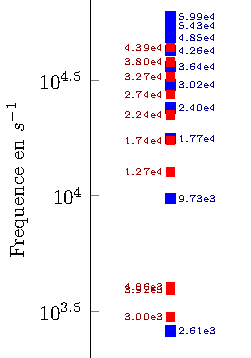
\includegraphics[height=6cm ,keepaspectratio]{Tikz/Frisedt/Freq.pdf} 
							\end{minipage}
						\end{figure}
						\begin{textblock}{6}[0,0](2,12)
							on ne trouve pas mieux de correspondance entre $\omega_0$ et les premiers modes de la POD
						\end{textblock}
						}
				\end{itemize}  % }
		\end{itemize}

	\end{frame}

%\section{Point de travail - avancement}

%\section{Questions soulevées}
%\begin{frame}
%$dt=$ \encircleR{200} \encircleB{100} \encircleK{50} \encircledR{25} \encircledB{10} \encircledK{5} $e^{-8}s$
%\end{frame}
\section{Dépouillement du cluster}
\begin{frame}
	Aberrations:
	\begin{figure}
		\only<1>{
						\hspace{-1cm}
						\begin{minipage}{0.45\linewidth}
						\FPeval{\result}{trunc((-1+\overlaynumber)*2 +1 :0)} 
							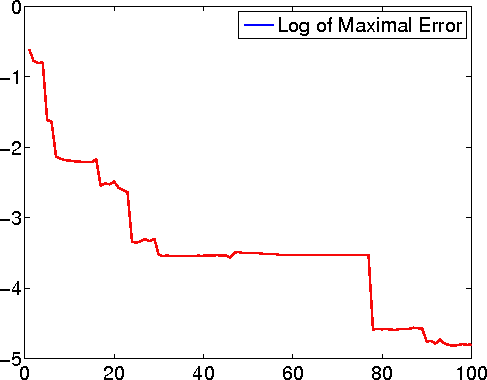
\includegraphics[width=6cm ,keepaspectratio]{Cluster2014_Erreur_cas_2_schem_3_Tcharge_250_Tstep_50_Transp.png}
							\caption{2014}
						\end{minipage}
						\hspace{0.7cm}
						\begin{minipage}{0.45\linewidth}
						\FPeval{\result}{trunc((-1+\overlaynumber)*2 +2 :0)} 
							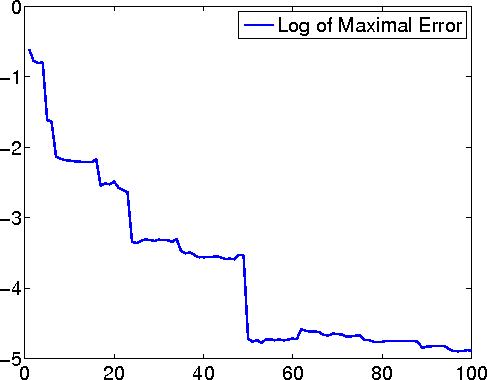
\includegraphics[width=6cm ,keepaspectratio]{Cluster2015_Erreur_cas_2_schem_3_Tcharge_250_Tstep_50_Transp.png}
							\caption{2015}
						\end{minipage}
			}
			\only<2>{
				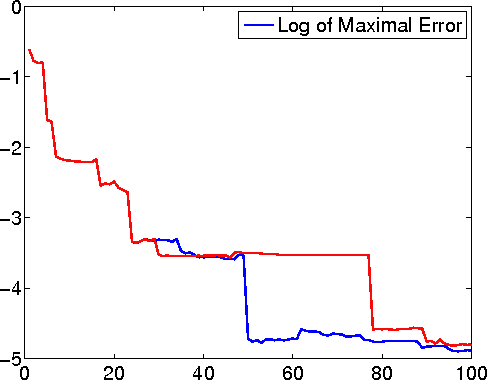
\includegraphics[width=6cm ,keepaspectratio]{ClusterMix_Erreur_cas_2_schem_3_Tcharge_250_Tstep_50_Transp.png}
			}
	\end{figure}
\end{frame}
	\begin{frame}
	\frametitle{Sortie de cluster}
			\only<1-3>{ \FPeval{\result}{trunc(2+\overlaynumber :0)} Charge Violente $T=4'000e^{-8}s$, Schema \result }
			\only<4-6>{ \FPeval{\result}{trunc(-1+\overlaynumber :0)} Charge Douce $T=25'000e^{-8}s$, Schema \result }
			\only<1-6>{
					\begin{figure}
						\hspace{-1cm}
						\begin{minipage}{0.45\linewidth}
						\FPeval{\result}{trunc((-1+\overlaynumber)*2 +1 :0)} 
							\includegraphics[trim=1.7cm 1cm 1cm 0.5cm, clip=true,width=6cm ,keepaspectratio]{Cluster/clusB\result.eps}
							\caption{Sinus}
						\end{minipage}
						\hspace{0.8cm}
						\begin{minipage}{0.45\linewidth}
						\FPeval{\result}{trunc((-1+\overlaynumber)*2 +2 :0)} 
							\includegraphics[trim=1.7cm 1cm 1cm 0.5cm, clip=true,width=6cm ,keepaspectratio]{Cluster/clusB\result.eps}
							\caption{SinusVerse}
						\end{minipage}
					\end{figure}
					\centering
					$dt=$ \encircleR{400} \encircleG{200} \encircleB{100} \encircleK{50} \encircledR{25} \encircledG{10} \encircledB{5} $e^{-8}s$
			}
			\only<7>{
			\framesubtitle{Conclusion}
			\begin{itemize}
				\item Solution PGD $\Rightarrow$ Soltion directe, quand $dt$ $\searrow$
					\begin{itemize}
						\FontReduce
						\item Abandonner $dt > 100 $
					\end{itemize}
				\item Convergence : Sinus $\sim>$ SinusVerse
					\begin{itemize}
						\FontReduce
						\item $\circ$ Rapidité de divergence
						\item $\circ$ Qualité solution à 100 modes
						\item $\sim$ Rapidité à stagnation
						\item $\bullet$ stagnations après les premiers modes
					\end{itemize}
			\end{itemize}
			}
	\end{frame}
\section{Constats et Remarques}
	\begin{frame}
	\FontReduceT
		\frametitle{Constats et Remarques}
		\begin{itemize}
			\only<1>{
			\item Utilisation du Cluster
				\begin{itemize}
					\item Résultat différents pour un même calcul:
						\begin{itemize}
							\item Cas divergent - Courbe d'erreur : 
							\\
							\begin{figure}
								\begin{minipage}{0.45\linewidth}
									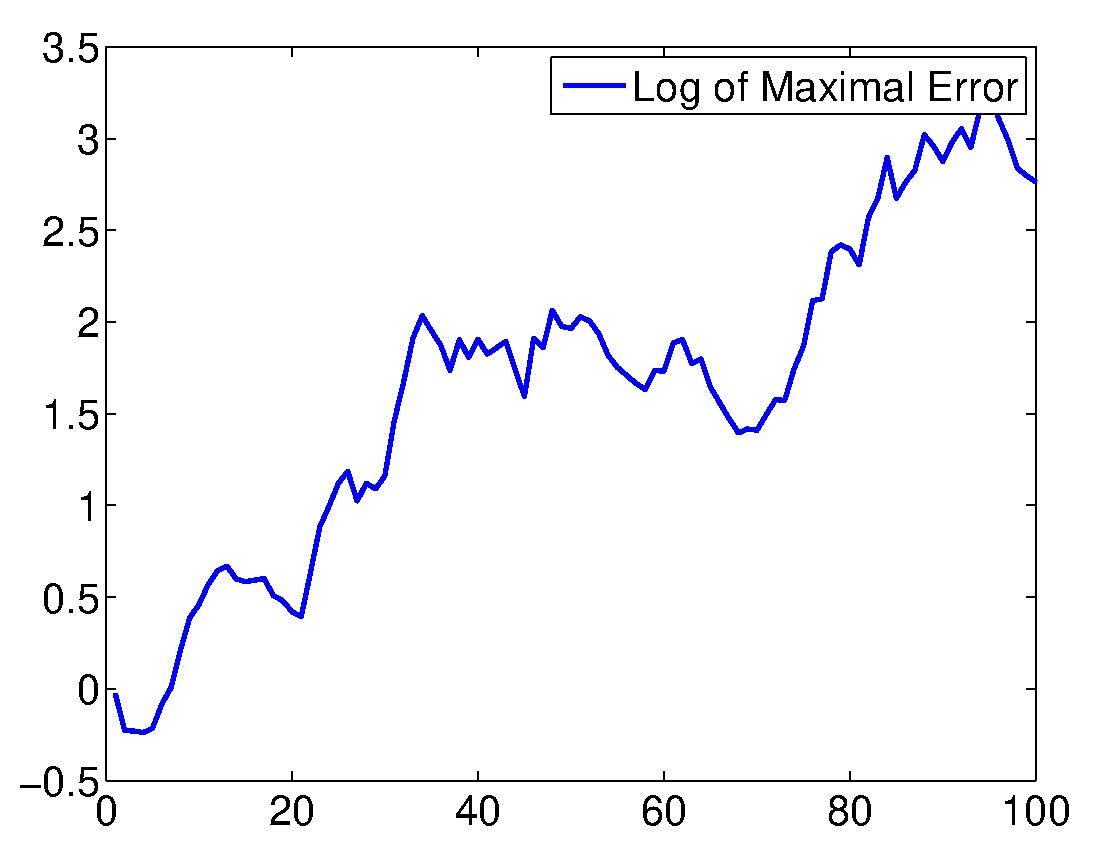
\includegraphics[width=3cm ,keepaspectratio]{matPGDErreur-Diverg-Cluster.eps}
									\caption{Sur le cluster}
								\end{minipage}
								\begin{minipage}{0.45\linewidth}
									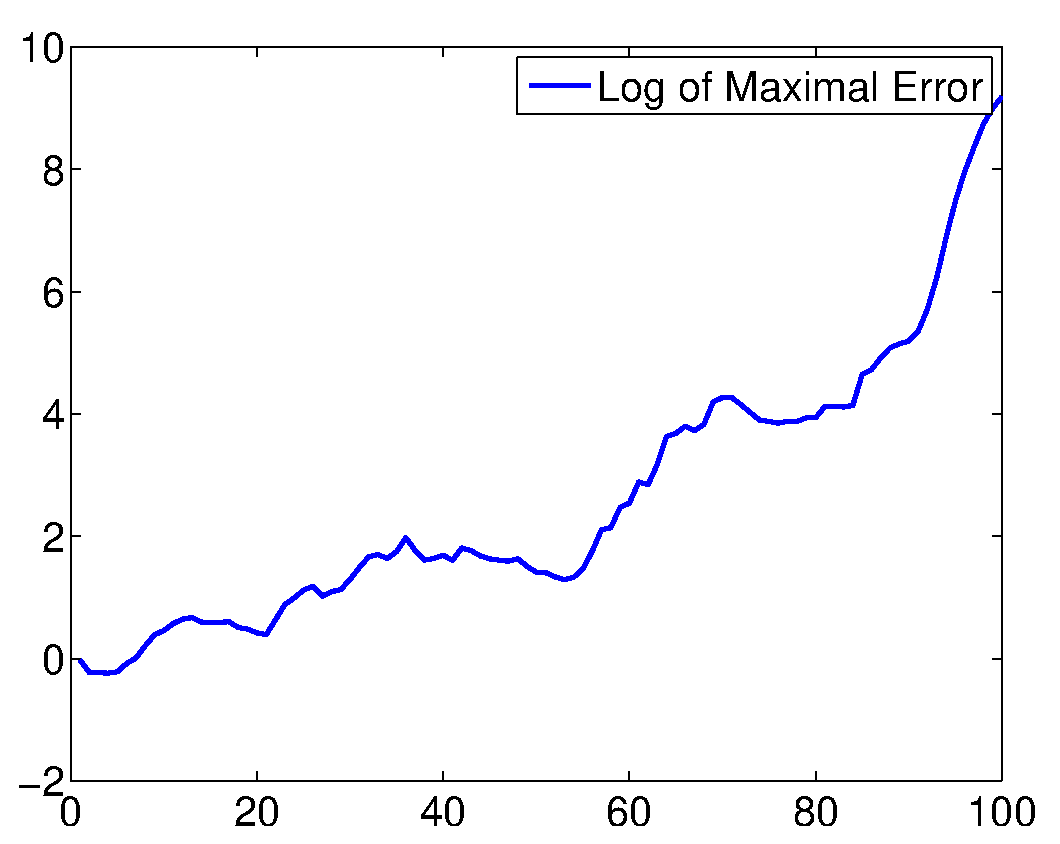
\includegraphics[width=3cm ,keepaspectratio]{matPGDErreur-Diverg-Local.eps}
									\caption{Sur mon Mac}
								\end{minipage}
							\end{figure}
							ceci pourrait être dû à la gestion de la précision des flottants sur des machines différentes.
							\item Cas convergent ??
						\end{itemize}
				\end{itemize}
				}
			\only<2>{
			\item Utilisation du Cluster - ce que j'attends du dépouillement
			\begin{itemize}
				\item Observer le rapprochement de la PGD par rapport à la résolution directe quand la discrétisation en temps est raffinée
					dans des cas plus ou moins violents et avec les différents schémas.
				\item Trancher entre SinusVerse et Sinus.				
				\item Faire les comparaison d'$\omega_0$ avec des cas au $dt$ faible
			\end{itemize}
				\begin{textblock}{5}[0,0](2,13)
					Les slides suivants était présentés lors de la réunion avec François.
				\end{textblock}
			}
			\only<3>{
			\item Les résultats sur masse-ressort cas SinuVerse - Différents amortissements et schémas
				\begin{itemize}
					\FontReduce
					\item $\xi = 0.7$
						\begin{itemize}
							\FontReduce
							\item Schéma 3 $\Rightarrow$ Convergence
							\item Schéma 4 et 5 $\Rightarrow$ Stagnation à $10^{-2.7}$
						\end{itemize}
					\item $\xi = 0.9$ (même en changeant $\alpha$)
						\begin{itemize}
							\FontReduce
							\item Schéma 3 $\Rightarrow$ ?
							\item Schéma 4 $\Rightarrow$ Convergence
							\item Schéma 5 $\Rightarrow$ Stagnation à $10^{-2.7}$
						\end{itemize}
					\item $\xi = 1.2$ (même en changeant $\alpha$)
						\begin{itemize}
							\FontReduce
							\item Schéma 3 $\Rightarrow$ ?
							\item Schéma 4 $\Rightarrow$ Convergence - Plus lente
							\item Schéma 5 $\Rightarrow$ Convergence très lente $10^{-0.8}$ à 20 modes
						\end{itemize}
				\end{itemize}
			\item Augmentation de l'amortissement sur problème poutre $\Rightarrow$ pas de résolution PGD. Divergence du premier point fixe.
				}
			\only<4-6>{
				\item Implémentation de la SVD dans le calcul des Modes
				\begin{itemize}
				}
			\only<4>{
					\item Avant d'appliquer la SVD
			\begin{figure}
				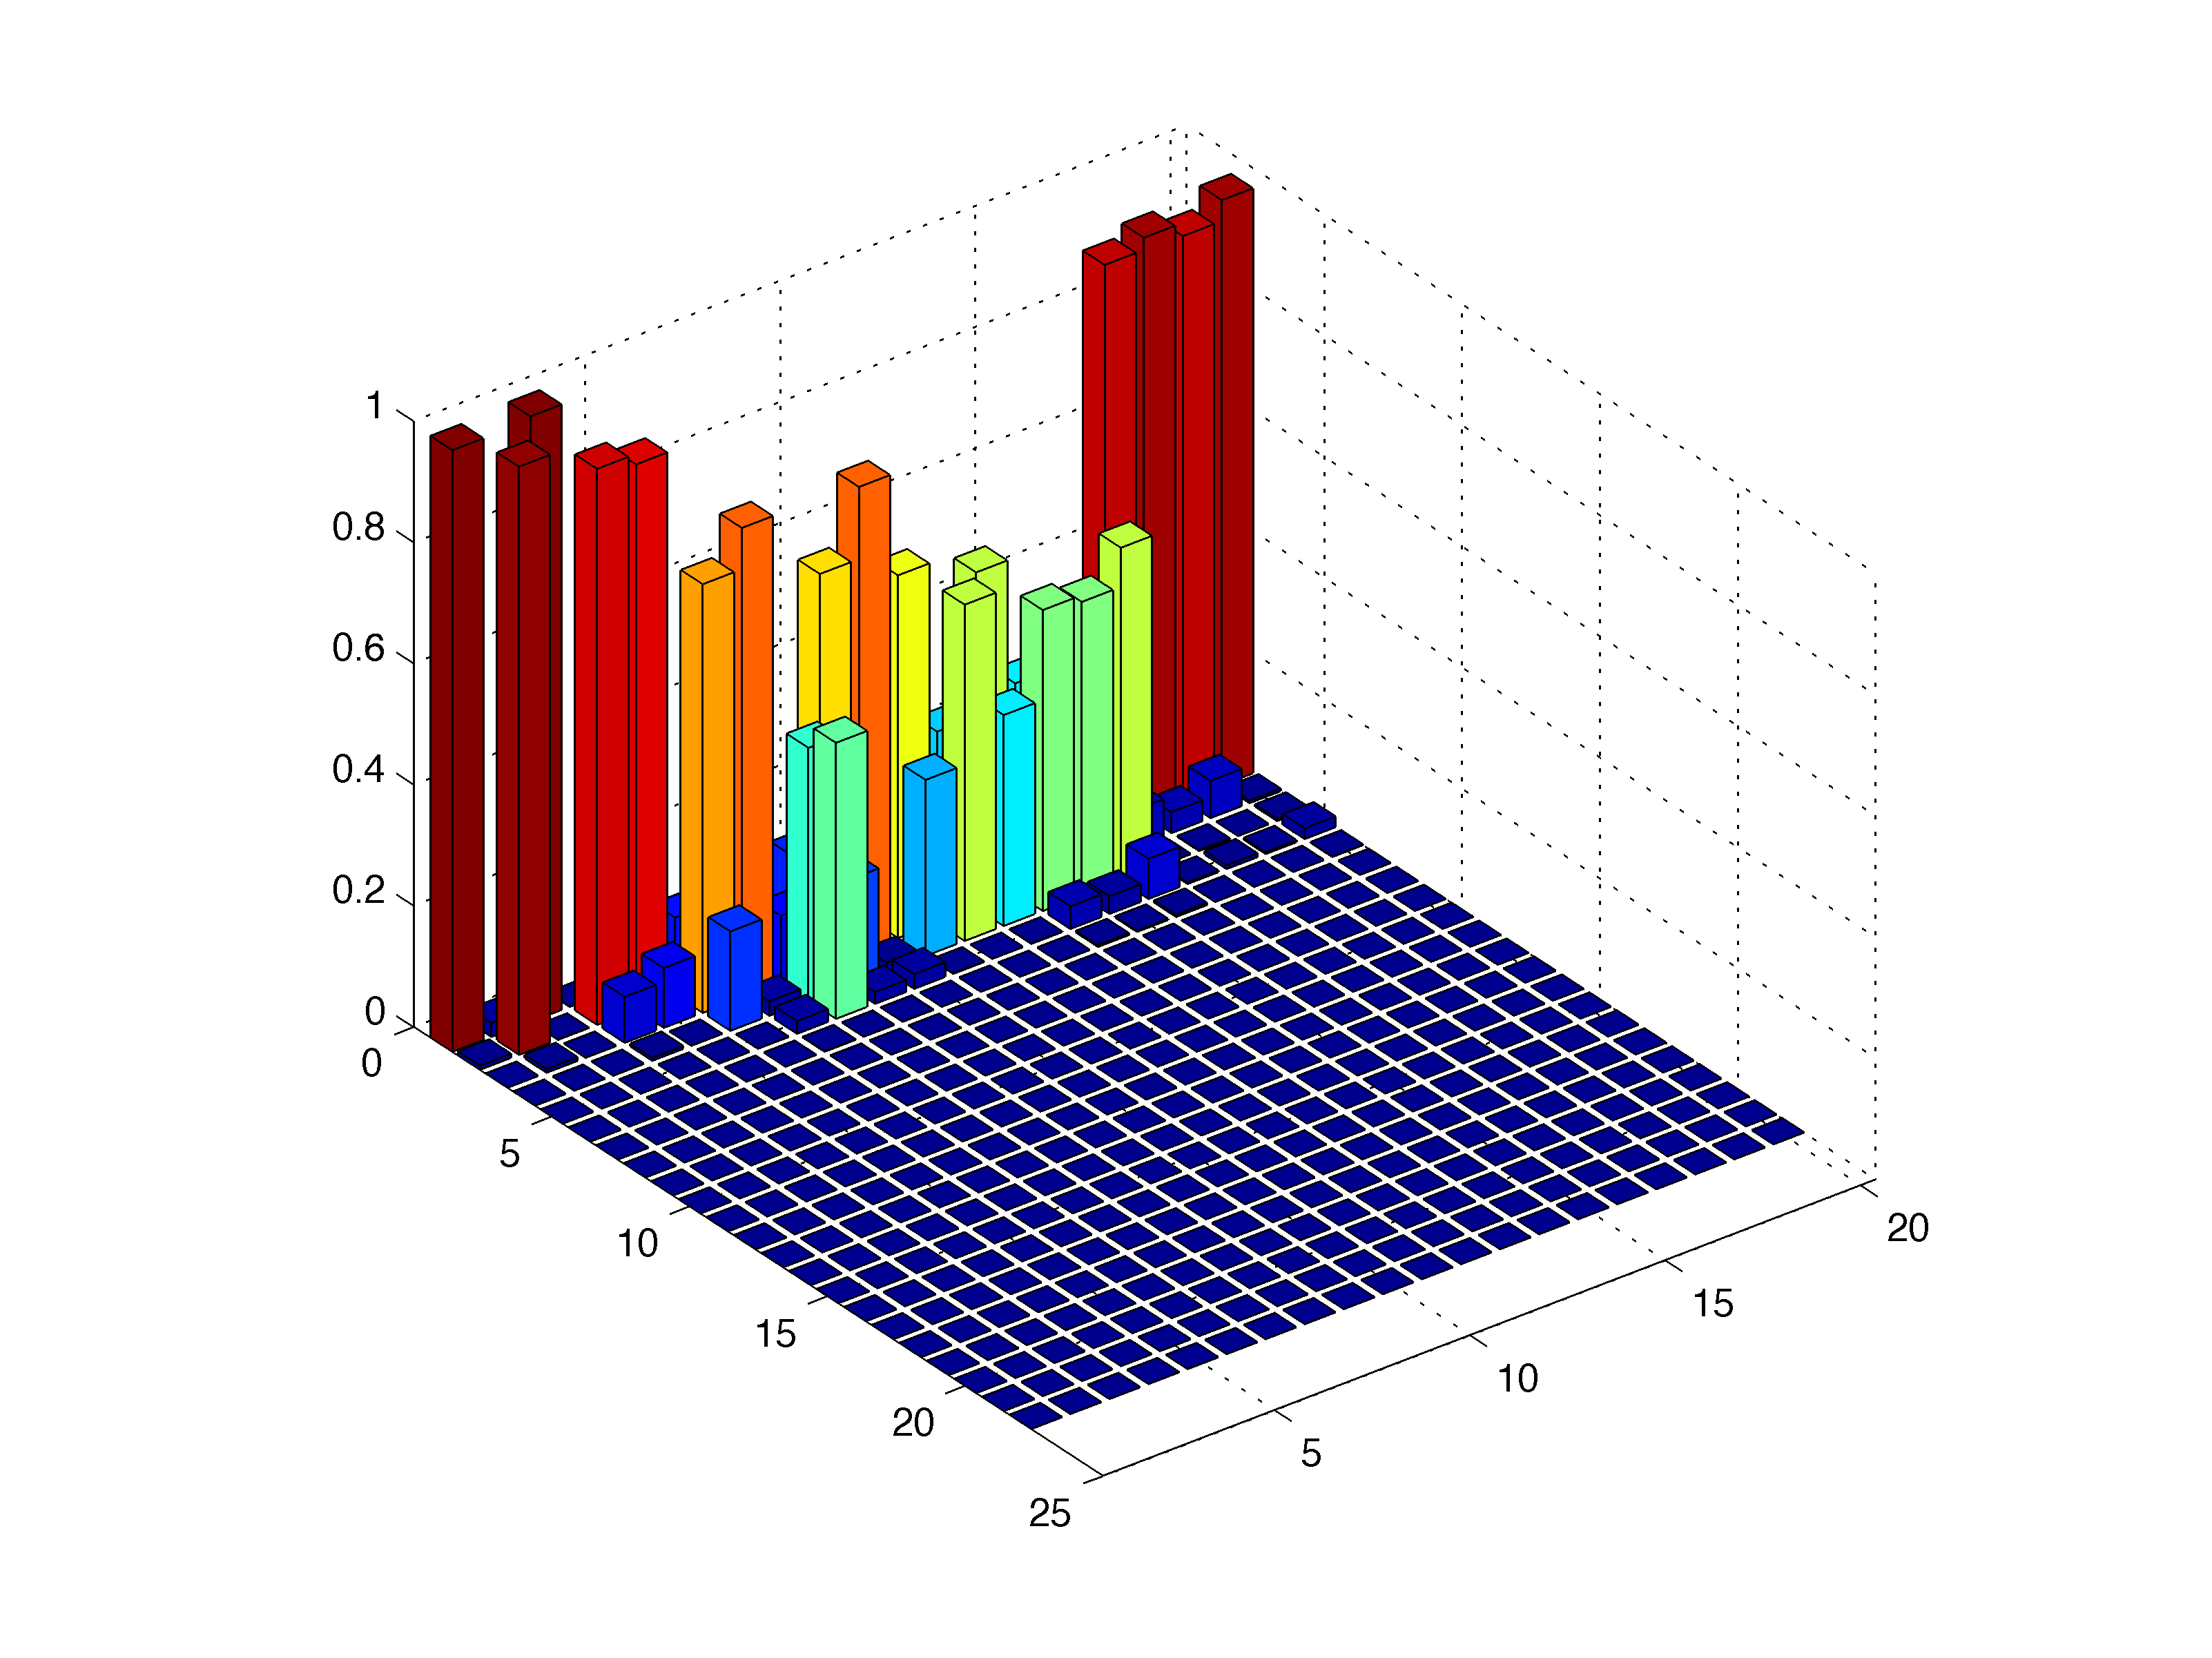
\includegraphics[width=0.5\linewidth ,keepaspectratio]{MAC_POD-PGD-Avant.png}				
				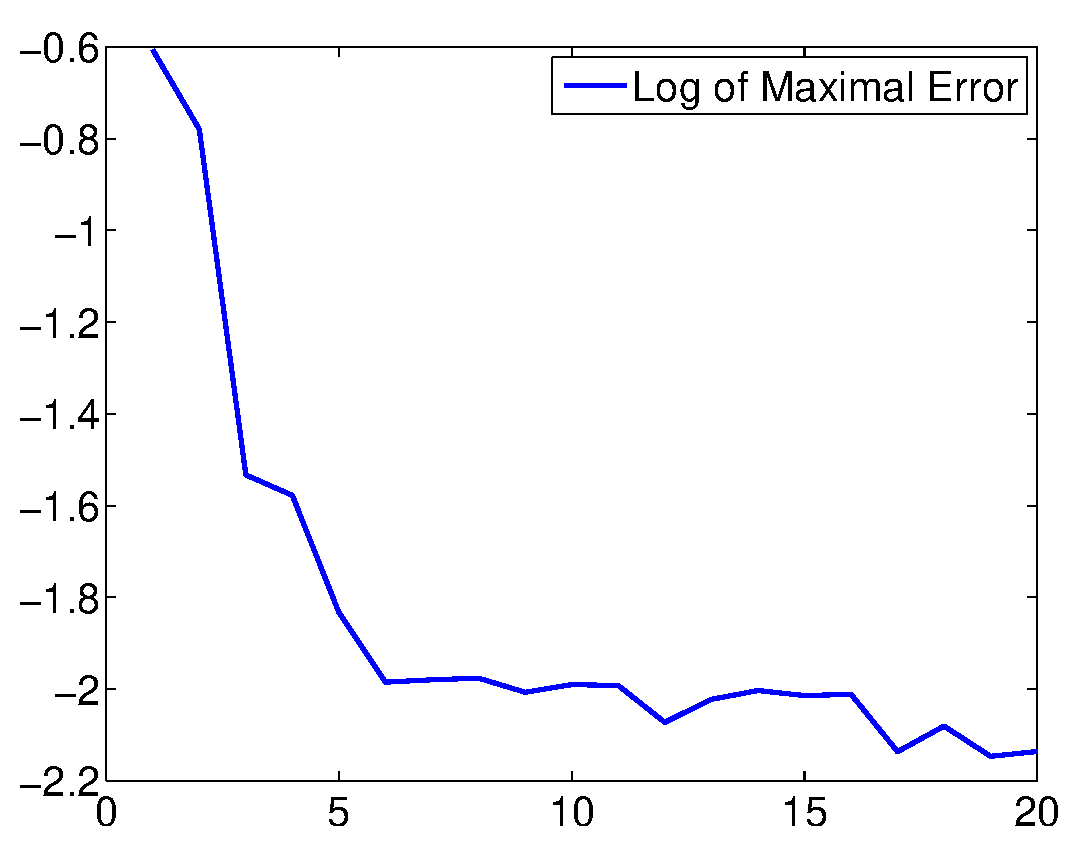
\includegraphics[width=0.5\linewidth ,keepaspectratio]{matPGDErreur-Avant.eps}	
			\end{figure}
			On calcule 20 modes PGD qui semblent de représenter que les premiers modes POD.
			}
			\only<5>{
					\item La SVD sur la Solution trouvée par PGD avec 20 couples, donne 10 nouveaux couples
			\begin{figure}
				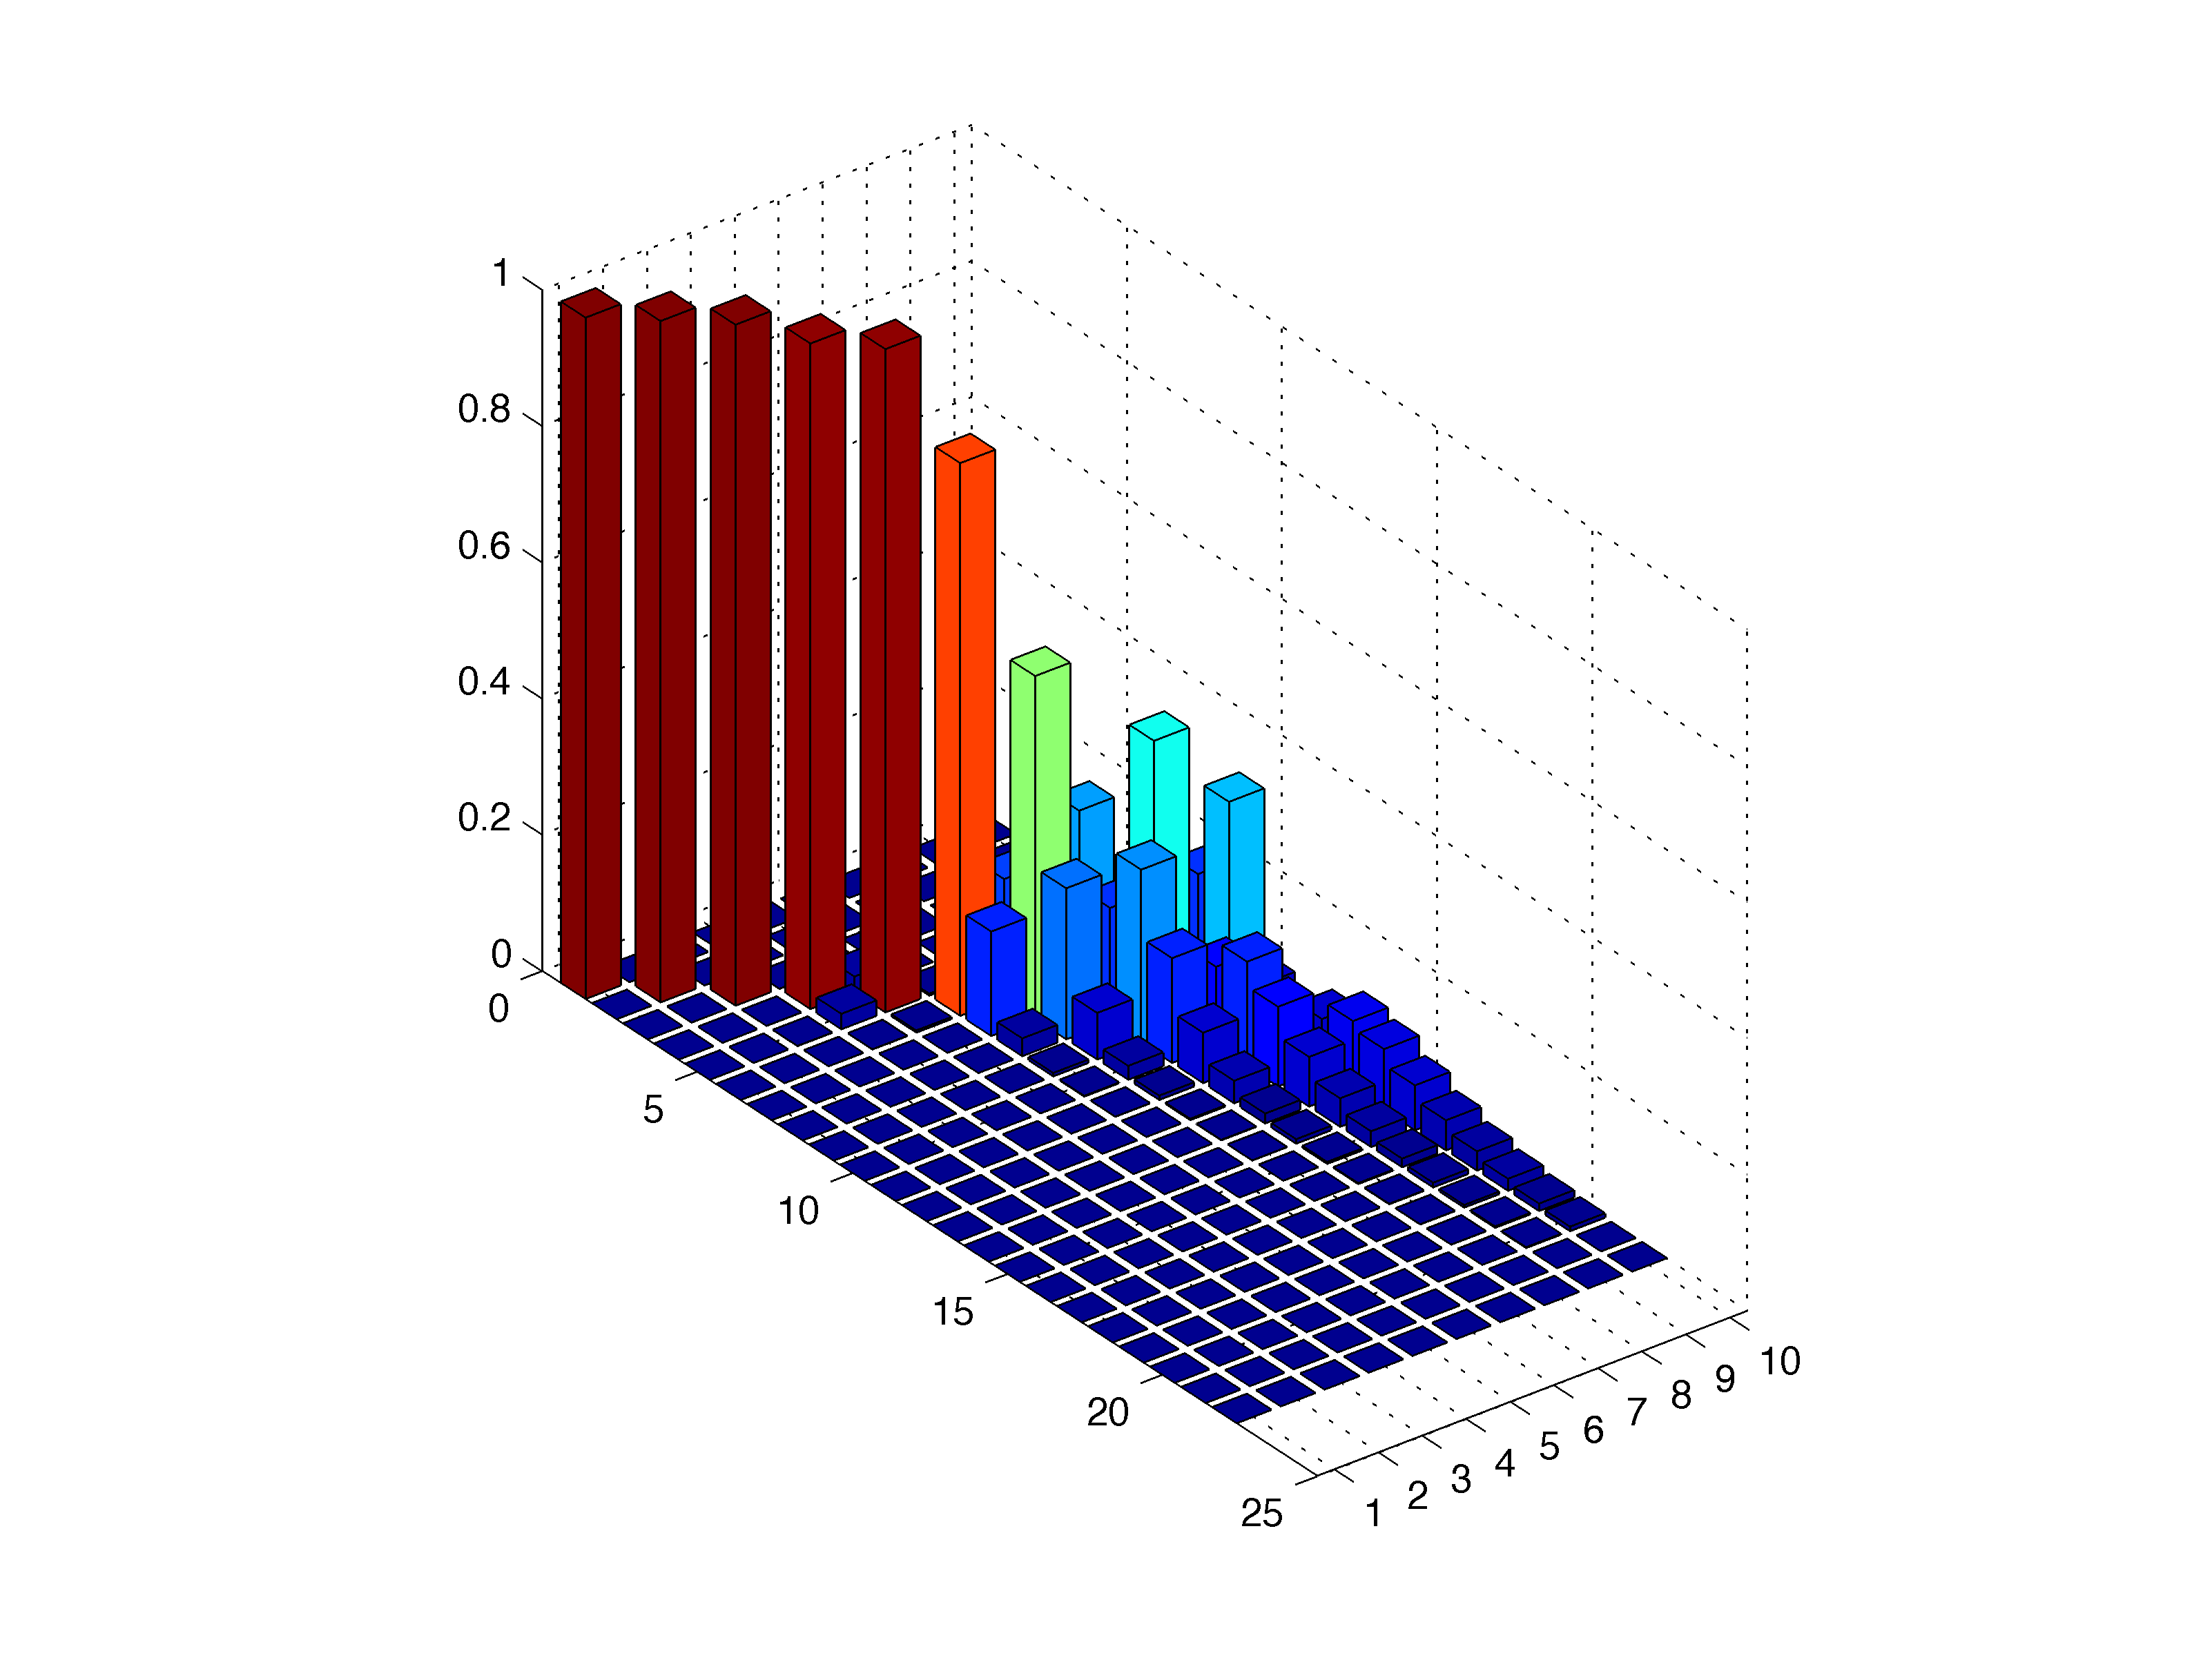
\includegraphics[width=0.5\linewidth ,keepaspectratio]{MAC_POD-PGD-apres.png}				
				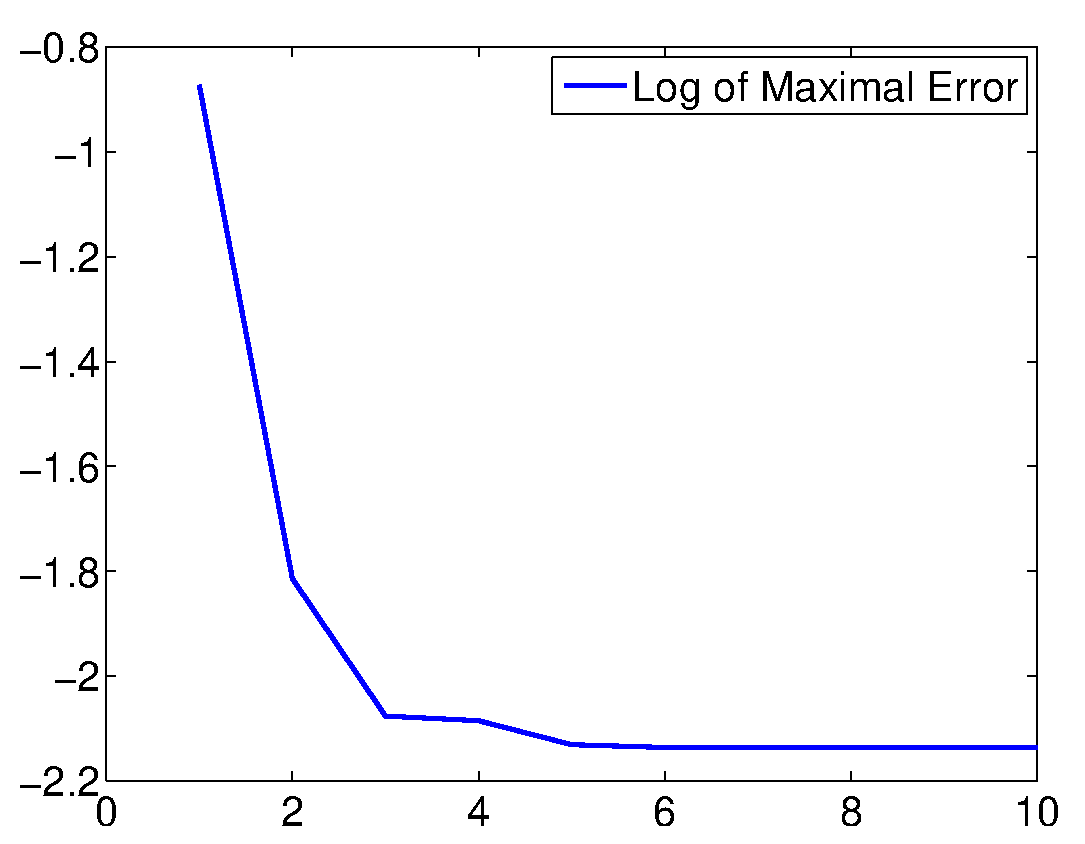
\includegraphics[width=0.5\linewidth ,keepaspectratio]{matPGDErreur-apres.eps}	
			\end{figure}
			On trouve les même modes que la POD et l'erreur décroit évidemment plus rapidement que précédemment.
			\\ Remarque: les modes trouvés au delà des 5-6 premiers semblent représenter une information qui n'apparaissait pas précédemment
			}
			\only<6>{
					\item Après l'application de la SVD
			\begin{figure}
				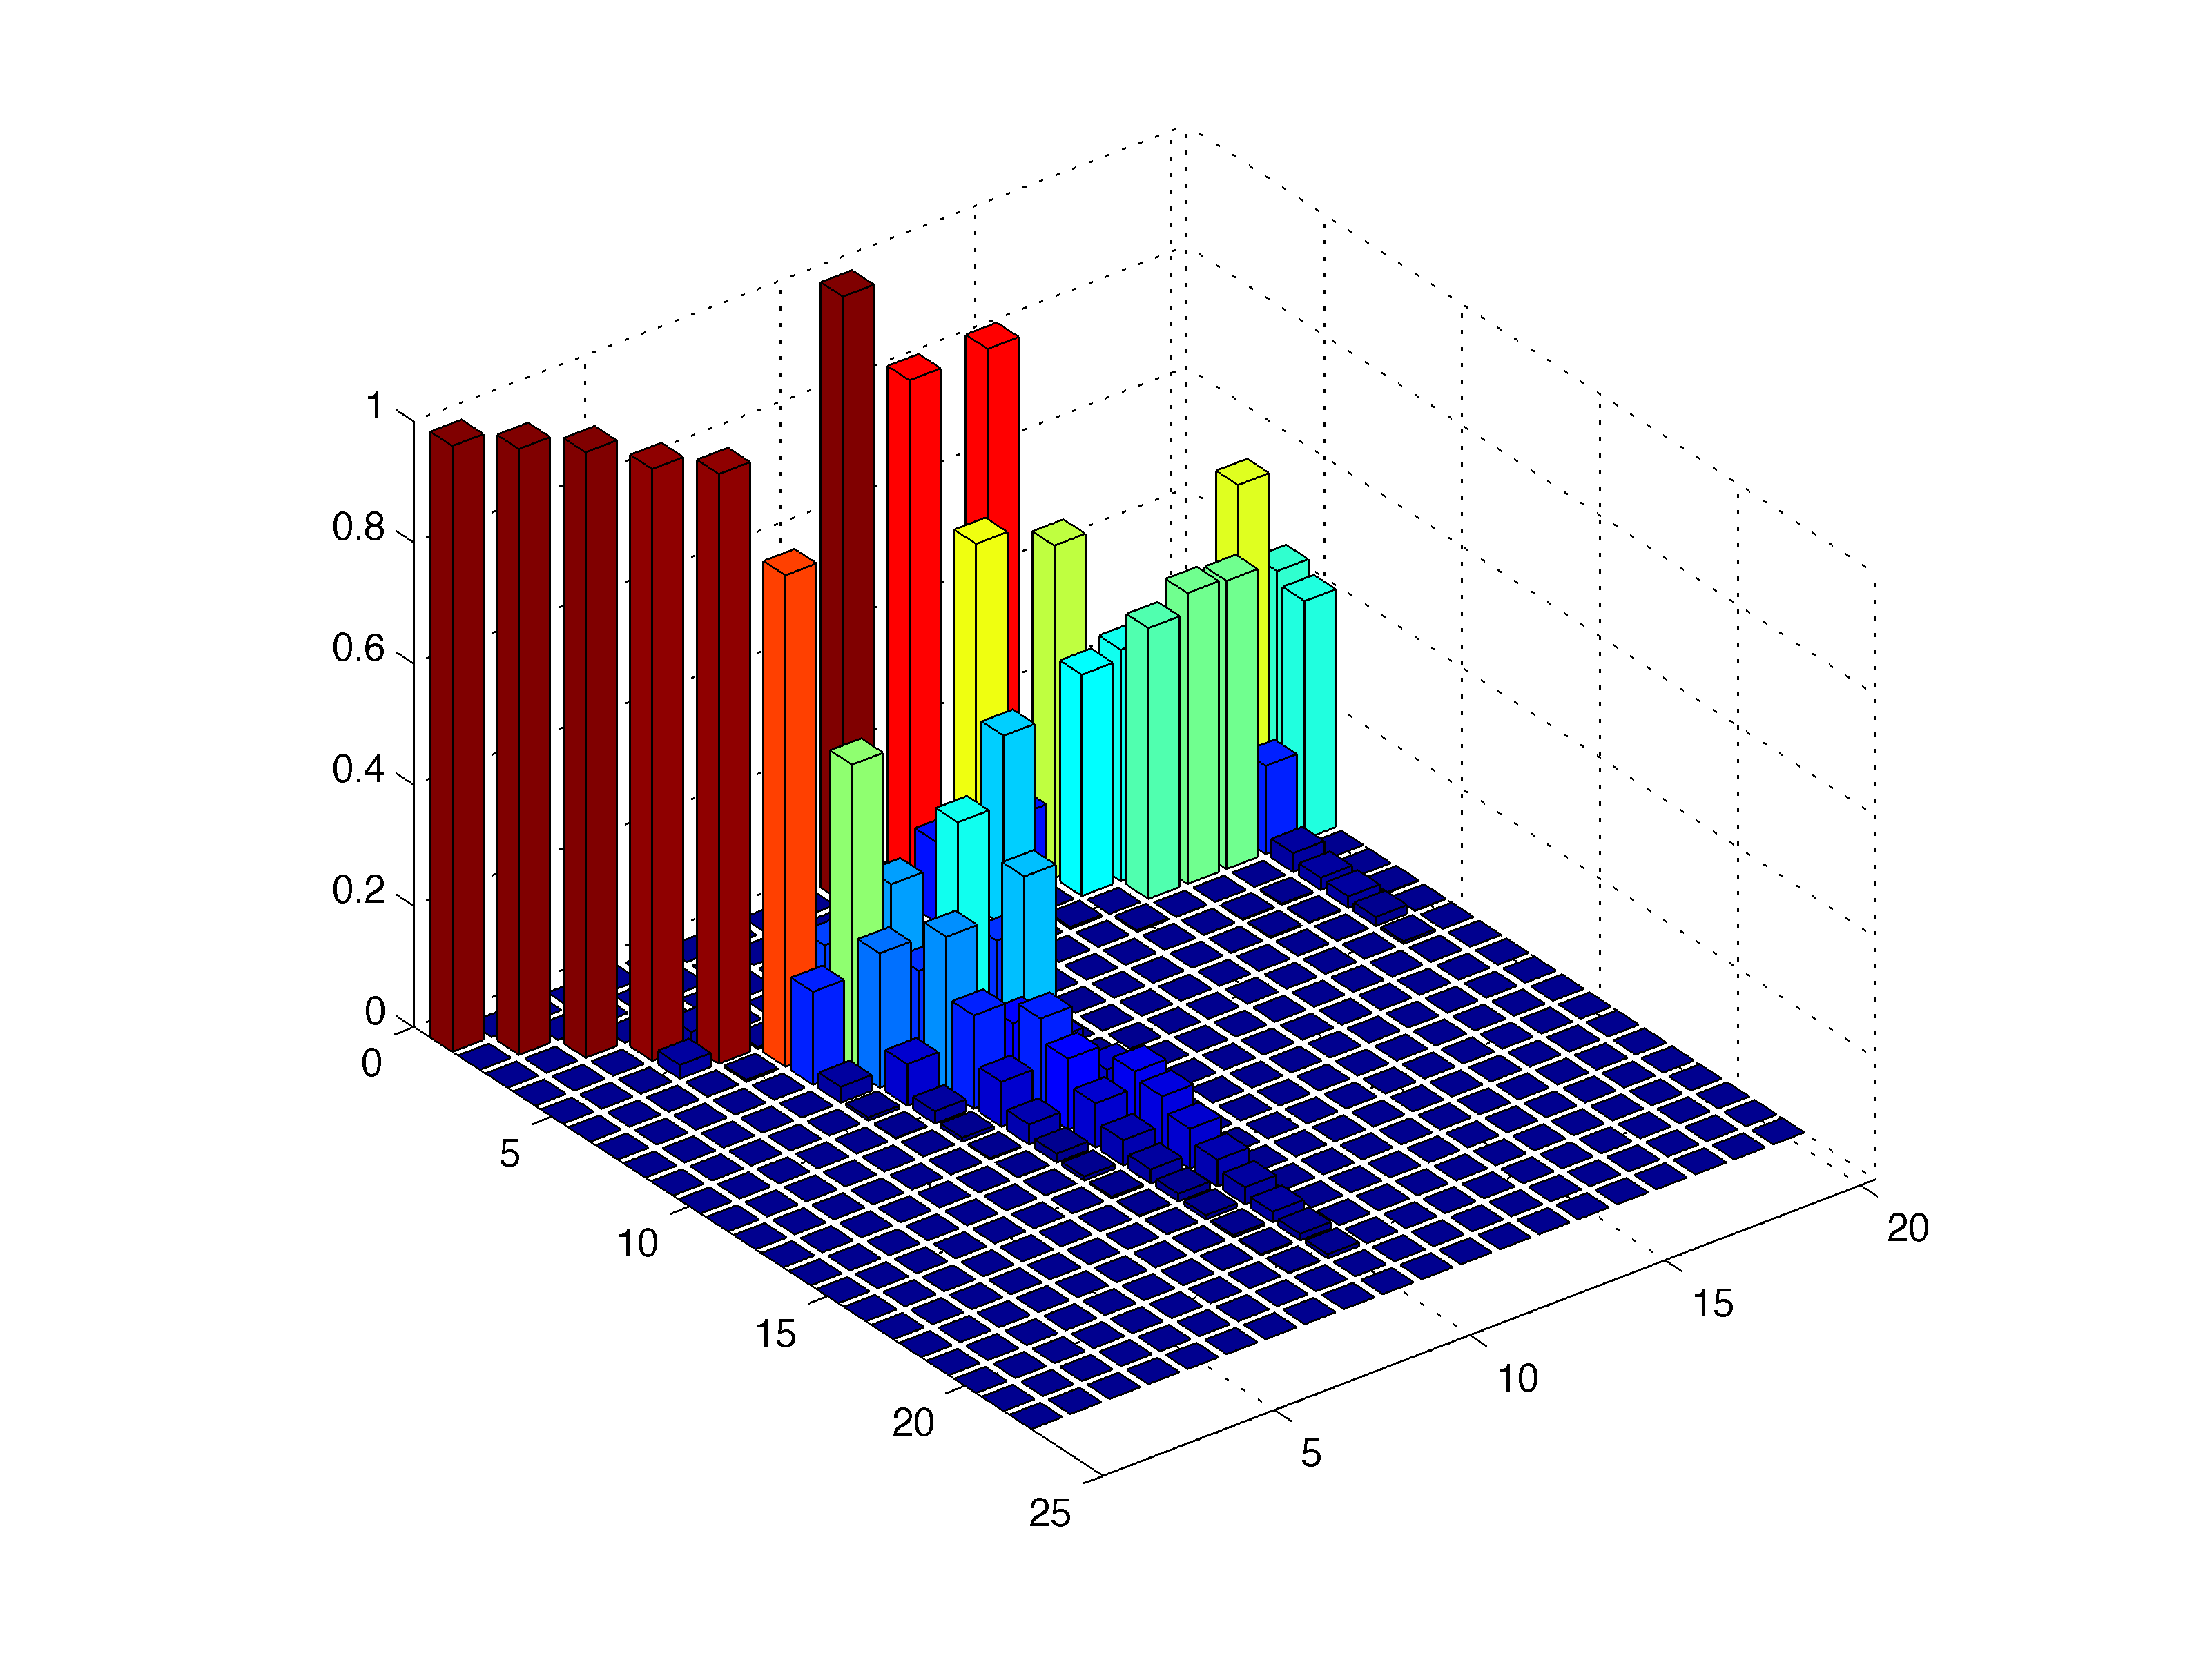
\includegraphics[width=0.5\linewidth ,keepaspectratio]{MAC_POD-PGD-continu.png}				
				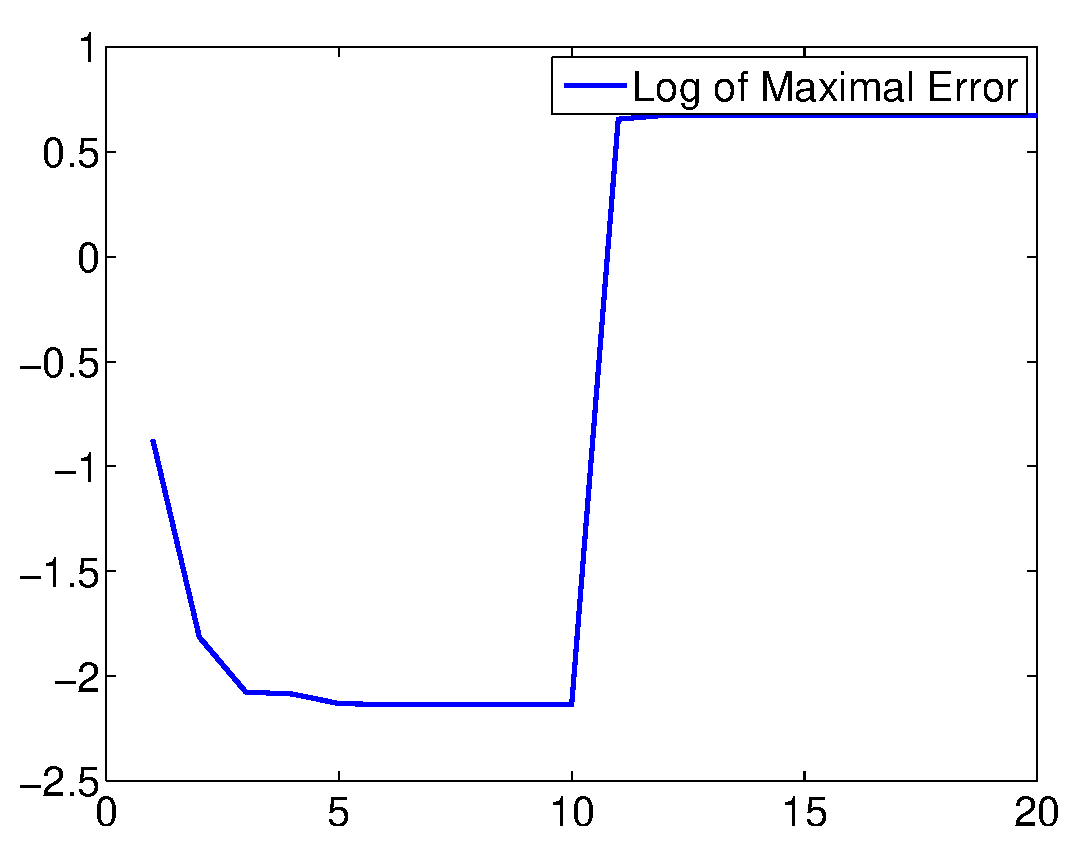
\includegraphics[width=0.5\linewidth ,keepaspectratio]{matPGDErreur-continu.eps}	
			\end{figure}
				Nouveaux modes trouvés incorrects - trop grand $\Rightarrow$ calcul de $g(t)$ faux,
					certainement de même origine que mes problèmes d'orthogonalisation.
			}
			\only<4-6>{
				\end{itemize}
				}
		\end{itemize}
	\end{frame}
	

%\section{Modifications dans le programme}
%	\begin{frame}
%		\frametitle{Modifications dans le programme}
%		\begin{itemize}
%			\item $\bullet$ Afficher les modes de POD redressés plutôt que la sortie de SVD
%			\item $\circ$ Utilisation de plusieurs non-linéarités
%				\begin{itemize}
%					\FontReduce
%					\item Le problème peut se présenter aussi avec une seule non-linéarité
%				\end{itemize}
%		\end{itemize}
%	\end{frame}
	
%\section{Idées}
%\subsection{Presudo-programme}
%\subsection{Cas test}
%\subsection{Equations}
%\section{Objectifs de travail}

%\section{Points blocants}
%
%	\begin{frame}
%	
%		\frametitle{Points blocants}
%		\begin{itemize}
%			\item PGD - TDG
%			\item Orthogonalisation
%			\item PGD \& Non-linéaire
%				\begin{itemize} 
%					\item Comment prendre en compte l'évolution de $ \mathbf{K} $ dans le problème en espace.
%				\end{itemize}
%			\item Absence d'éléments de comparaison pour les résultats non-linéaire.
%		\end{itemize}
%	
%	\end{frame}

%\section{Questions}
%
%	\begin{frame}
%	
%		\frametitle{Questions}
%		
%		\begin{itemize}
%			\item Comment dans le calcul de $g(t)$ est influencé par la norme de $f(x)$?
%			\begin{itemize}
%				\item Problème en temps : équation proportionnelle à $f_q$.
%			\end{itemize}
%		\end{itemize}
%	
%	\end{frame}
	
\section{Programme de travail}

	\begin{frame}
	
		\frametitle{Programme de travail}
		
		\begin{itemize}
			\item Réunion MECASIF 16 Janvier.
		\end{itemize}
	
	\end{frame}

\end{document}
% ---------------------------------------------------------------------
